\documentclass[12pt,english]{beamer}
\usepackage[utf8]{inputenc}
\usepackage[T1]{fontenc}
\usepackage{booktabs}
\usepackage{babel}
\usepackage{graphicx}
\usepackage{csquotes}
\usepackage{xcolor}
\usepackage{listings} 
 
\lstset{basicstyle=\ttfamily\footnotesize,
  showstringspaces=false,
  commentstyle=\color{red},
  keywordstyle=\color{blue},
language=bash,
frame=single,
morekeywords={git,mkdir,status,touch,add,config}
}

\usepackage[sfdefault]{plex-sans}
\usetheme[progressbar=frametitle]{metropolis}           % Use metropolis theme
 
\title{Some GIT Basics}
\date{\today}
\author{Dr. Uwe Ziegenhagen}
\institute{www.uweziegenhagen.de}
 
\makeatletter
\setlength{\metropolis@titleseparator@linewidth}{1pt}
\setlength{\metropolis@progressonsectionpage@linewidth}{1pt}
\setlength{\metropolis@progressinheadfoot@linewidth}{1pt}
\makeatother
 
\begin{document}
 
\begin{frame}
	 \maketitle
\end{frame}
 
\begin{frame}
\frametitle{Content}

\tableofcontents
\end{frame}

\section{Introduction}

\begin{frame}
\frametitle{Introduction}
 
\begin{itemize}
\item \enquote{Git is a free and open source distributed version control system designed to handle everything from small to very large projects with speed and efficiency. }
\item Version control systems track changes to files and allow you to go back to earlier versions thus creating backups as well.
\item Git is not the first or only available version control system (VCS): CVS, Bitbucket, and Subversion are wellknown
\item Git was developed by the Linux creator Linus Torvalds to maintain the Linux kernel
\end{itemize}
\end{frame}
 
\begin{frame}
\frametitle{Centralized versus Distributed VCS}

\begin{itemize}
\item Subversion is a centralized vcs, it uses a central server. Only this server has the full history of all files
\item All developers get special snapshots from this server.
\item Backing up the server is essential!
\item Git is a distributed vcs, so all clients (developers) have the complete repository on their machines. 
\item I personally used Subversion for a long time (and still use it for some projects) but mostly have migrated to Github.
\item Github = a central platform where I can put my projects, but not the \enquote{central server} like with Subversion
\end{itemize}
\end{frame}

\begin{frame}
\frametitle{Working with Git}

In the following we will look as various use cases for working with Git

\begin{itemize}
\item Create new repositories\footnote{The project structure you manage with Git}
\item Add files to the repository
\item Making changes to the repository
\item 
\end{itemize}

Remark: Git can be quite complex, but normally you need only a few commands.

\end{frame}

\section{MinGW Basics}

\begin{frame}
\frametitle{Running Git}

\begin{itemize}
\item You find Git 2.28 on your desktop
\item When you start it you land here:
\end{itemize}

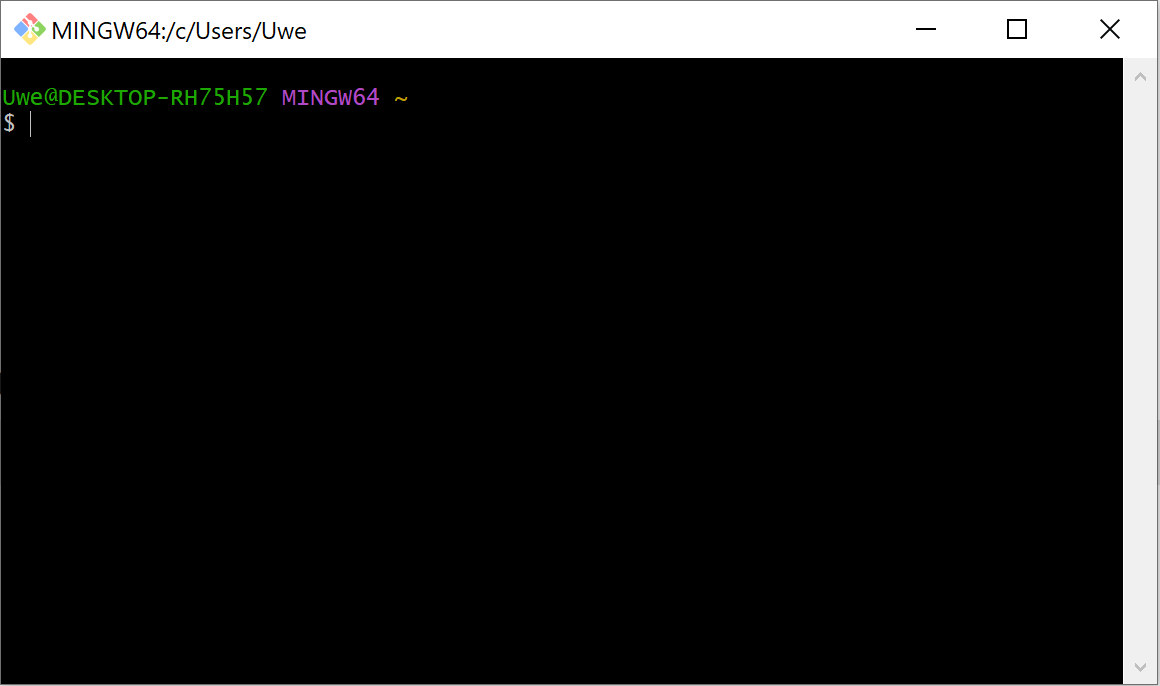
\includegraphics[width=\textwidth]{mingw-01}
\end{frame}
 
\begin{frame}
\frametitle{MinGW}

\begin{itemize}
\item MinGW = Minimal GNU\footnote{\enquote{GNU is not Unix} = Open-Source stuff} for Windows
\item A shell that ports many Unix/Linux tools to Windows
\item This is not Git, Git is just a commandline tool that can be used within MinGW
\item It contains a few Linux tools as well
\item To move in this MinGW environment you need to use Linux commands
\end{itemize}
\end{frame}

\begin{frame}
\frametitle{Basic MinGW commands}

\begin{description}
\item [pwd] In which directory are we?
\item [ls] List all files and folders
\item [cd] go to some specific directory
\item [mkdir] create a new directory
\end{description}

Remarks:

\begin{itemize}
\item There are no drive letters in MinGW
\item \texttt{/} is the root directory
\item Windows drive letters are (invisible) directories below this root directory
\item so \texttt{cd /c} takes you to the C:\textbackslash directory
\end{itemize}

\end{frame}

\section{Git}

\begin{frame}[containsverbatim]
\frametitle{Create new Repositories}

Create a directory, change to that directory and init the repository. The directory may already contains some files

\begin{lstlisting}
cd /e # go to the e: drive

mkdir myfirstgitrepo # create empty directory

cd myfirstgitrepo #  go to the directory

git init . # create repo (with a 'master' branch)
\end{lstlisting}

\end{frame}

\begin{frame}[containsverbatim]
\frametitle{git status}

Use \texttt{git status} whenever you want to know something about the current state of the repository

\begin{lstlisting}
Uwe@DESKTOP MINGW64 /e/myfirstgitrepo (master)
$ git status
On branch master

No commits yet

nothing to commit (create/copy files and use
"git add" to track)
\end{lstlisting}

\end{frame}

\begin{frame}[containsverbatim]
\frametitle{Adding files to the Repository 1} % create/copy files and use "git add" to track

\begin{lstlisting}
$ touch README.MD # creates an empty file

$ git status
On branch master

No commits yet

Untracked files:
(use "git add <file>..." to include in what will 
be committed)
        README.MD

nothing added to commit but untracked files 
present (use "git add" to track)
\end{lstlisting}

\end{frame}


\begin{frame}[containsverbatim]
\frametitle{Adding files to the Repository 2} 

\begin{lstlisting}
$ git add README.MD # add file to staging area

$ git add -A # add all files to staging area
# not added to repository

$ git reset # remove everything from the
# staging area

$ git commit -m "My message" # Don't forget!!!
\end{lstlisting}

\end{frame}


\begin{frame}[containsverbatim]
\frametitle{Adding files to the Repository 3} 

\begin{lstlisting}
$ git commit -m "Initial commit"
Author identity unknown

*** Please tell me who you are.

Run

  git config --global user.email "you@examp.de"
  git config --global user.name "Your Name"

to set your account's default identity.
Omit --global to set the identity only in this 
repository.

fatal: unable to auto-detect email address (got 
'Uwe@DESKTOP-RH75H57.(none)')
\end{lstlisting}

\end{frame}


\begin{frame}[containsverbatim]
\frametitle{Adding files to the Repository 4} 




\begin{lstlisting}[basicstyle=\ttfamily\scriptsize]
Uwe@DESKTOP MINGW64 /e/myfirstgitrepo (master)
$ git config --global user.email "ziegenhagen@gmail.com"

Uwe@DESKTOP MINGW64 /e/myfirstgitrepo (master)
$ git config --global user.name "Uwe Ziegenhagen"

Uwe@DESKTOP MINGW64 /e/myfirstgitrepo (master)
$ git commit -m "Initial commit"
[master (root-commit) acb9d75] Initial commit
 1 file changed, 0 insertions(+), 0 deletions(-)
 create mode 100644 README.MD

Uwe@DESKTOP MINGW64 /e/myfirstgitrepo (master)
$ git status
On branch master
nothing to commit, working tree clean
\end{lstlisting}

Now we have a file under version control! Yippie!

\end{frame}

\begin{frame}
\frametitle{A Word of Warning!}

\begin{itemize}
\item When you omit the commit message, Git takes you to vim (VI \enquote{improved}) to allow you to enter it
\item VIM = very powerful editor with strange user interface
\item VIM uses special modes and is (almost) keyboard-only
\end{itemize}

Let's edit our file and commit it\ldots 

You can use e.\,g. \texttt{nano} the edit the file.

\end{frame}

\begin{frame}
\frametitle{Editing the file with \texttt{nano README.MD}}

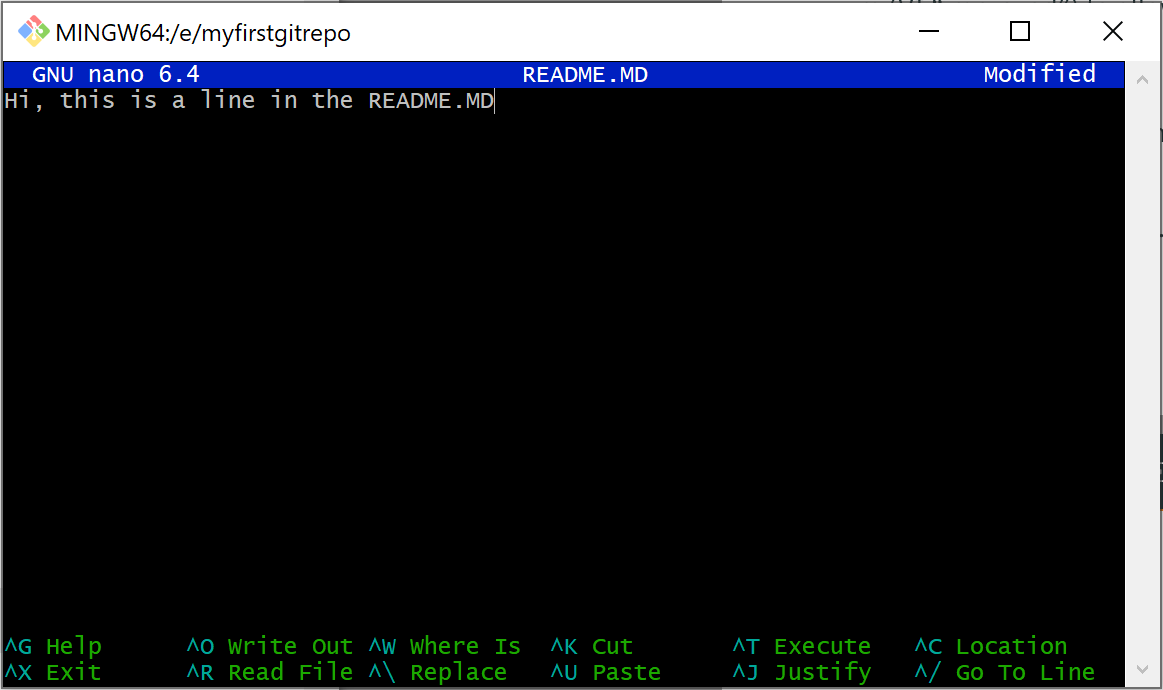
\includegraphics[width=\textwidth]{nano-edit}

\begin{itemize}
\item The circumflex means the Ctrl-key
\item So Ctrl-O saves the file, Ctrl-X exits \texttt{nano}
\end{itemize}

\end{frame}



\begin{frame}[containsverbatim]
\frametitle{Escape from VIM Hell\ldots -- Part 1} 

\begin{lstlisting}[basicstyle=\ttfamily\scriptsize]
Uwe@DESKTOP MINGW64 /e/myfirstgitrepo (master)
$ git status
On branch master
Changes not staged for commit:
  (use "git add <file>..." to update what will be committed)
  (use "git restore <file>..." to discard changes in working 
  directory)
        modified:   README.MD

no changes added to commit (use "git add" and/or
 "git commit -a")
\end{lstlisting}

Git notices that we changed a file, that is under version control

\end{frame}

\begin{frame}[containsverbatim]
\frametitle{Escape from VIM Hell\ldots -- Part 2} 

\begin{itemize}
\item We add the file to the commit stage
\item you can ignore the LF warning. It just means that \texttt{nano} used Unix-style line endings (\texttt{\textbackslash n}) in the file, for the repository however Windows line endings (\texttt{\textbackslash r\textbackslash n})
\end{itemize}

\begin{lstlisting}[basicstyle=\ttfamily\scriptsize]
Uwe@DESKTOP-RH75H57 MINGW64 /e/myfirstgitrepo (master)
$ git add README.MD
warning: in the working copy of 'README.MD', LF will be 
replaced by CRLF the next time Git touches it
\end{lstlisting}

Remarks: \texttt{\textbackslash n} means Line Feed-Character,  \texttt{\textbackslash r\textbackslash n} means Carriage Return + Line Feed. Helpful to know when working with text files.


\end{frame}



\begin{frame}[containsverbatim]
\frametitle{Escape from VIM Hell\ldots -- Part 3} 

We briefly check the status

\begin{lstlisting}[basicstyle=\ttfamily\scriptsize]
$ git status
On branch master
Changes to be committed:
  (use "git restore --staged <file>..." to unstage)
        modified:   README.MD
\end{lstlisting}

and commit it without specifying the message parameter

\begin{lstlisting}[basicstyle=\ttfamily\scriptsize]
$ git commit
\end{lstlisting}

Which takes us to eternal pain, the VIM!!!


\end{frame}

\begin{frame}
\frametitle{Escape from VIM Hell\ldots -- Part 4}

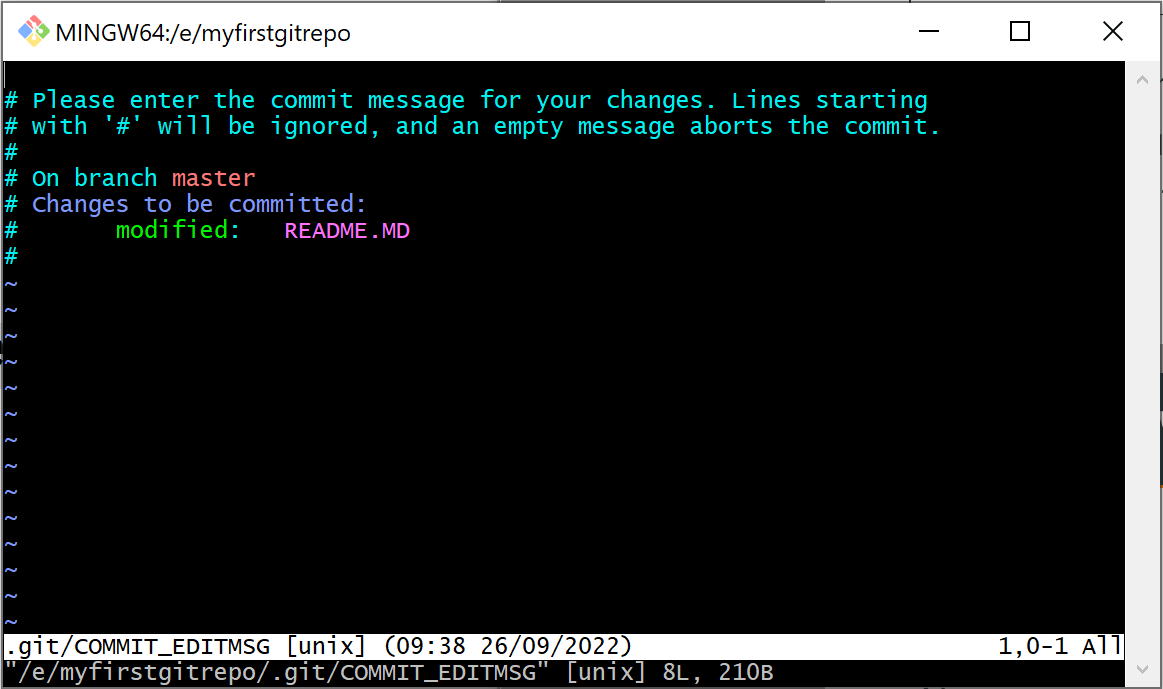
\includegraphics[width=\textwidth]{vim-hell}

\end{frame}

\begin{frame}
\frametitle{Escape from VIM Hell\ldots -- Part 5}

\begin{itemize}
\item \texttt{ESC}~\texttt{:}~\texttt{q} lets you exit without specifying a message, but you do not commit then.
\item \texttt{ESC}~\texttt{:}~\texttt{q}~\texttt{!} lets you exit without specifying a message if you typed anything, but you do not commit then.
\end{itemize}
\end{frame}

\begin{frame}
\frametitle{Display the commit history with \texttt{git log}}

\begin{itemize}
	\item \texttt{git log} for the history of commits
\item \texttt{git log -p} including the the full diff\footnote{diff = differences between file in the \texttt{diff} format}
\end{itemize}

\begin{center}
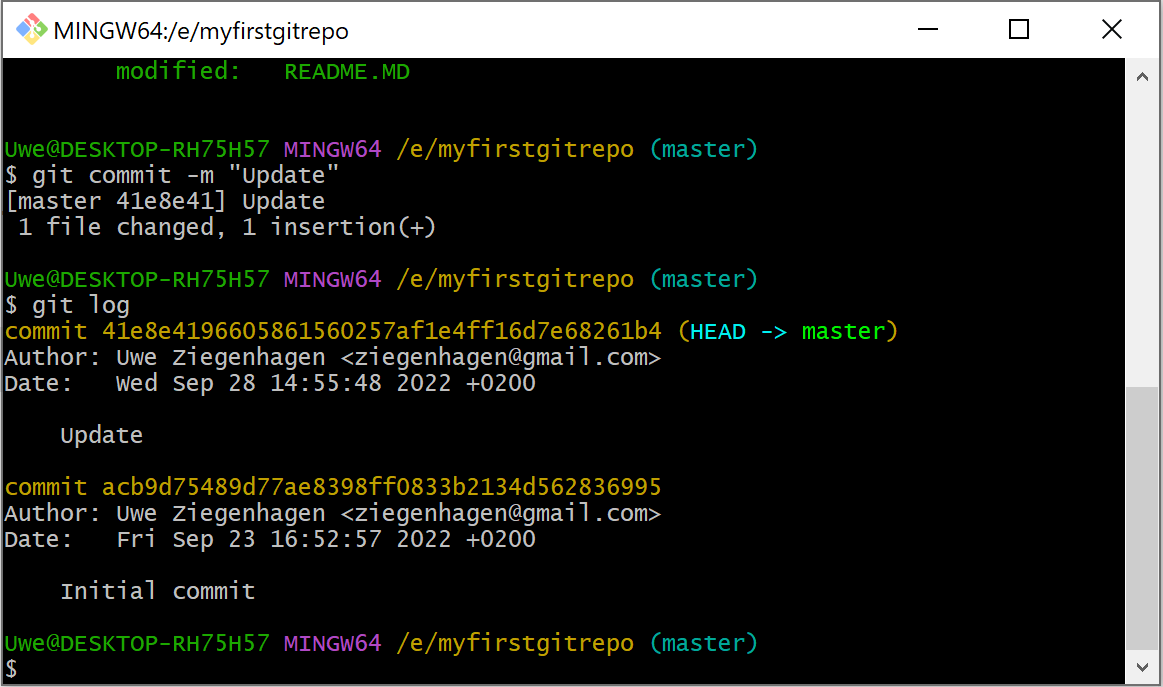
\includegraphics[width=0.75\textwidth]{gitlog}
\end{center}

\end{frame}

\begin{frame}
\frametitle{Example for \texttt{git log -p}}

\begin{center}
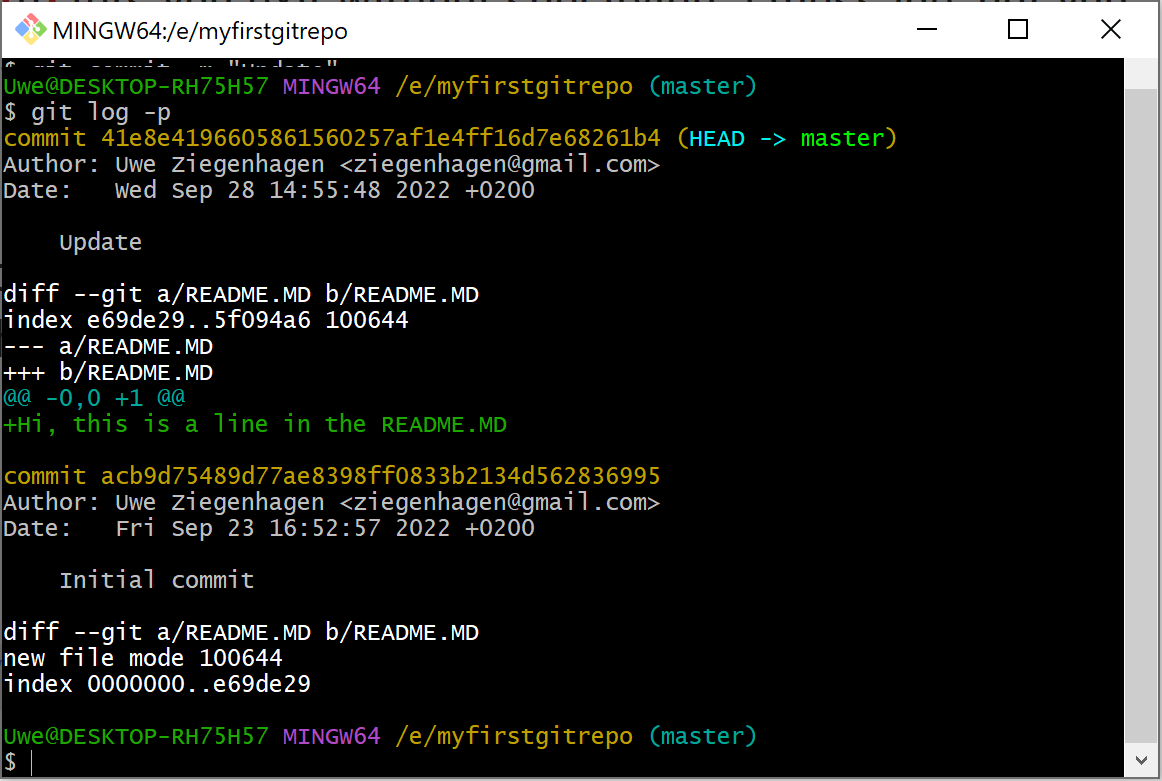
\includegraphics[width=\textwidth]{gitlogp}
\end{center}

\end{frame}

\begin{frame}
\frametitle{Get back to earlier versions 1}

\begin{itemize}
\item Let us assume we have this line in the old file
\end{itemize}

\begin{center}
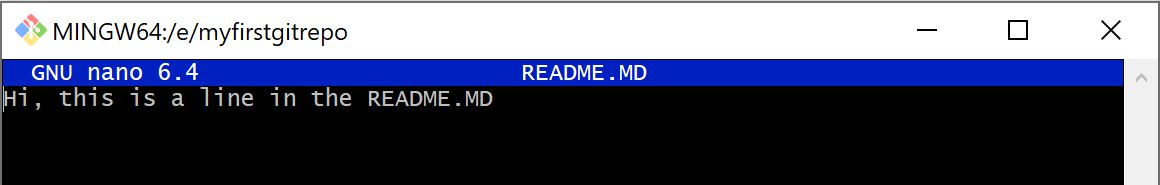
\includegraphics[width=\textwidth]{getback-1}
\end{center}

and have changed it (and added it to the staging area and commited it) 

\begin{center}
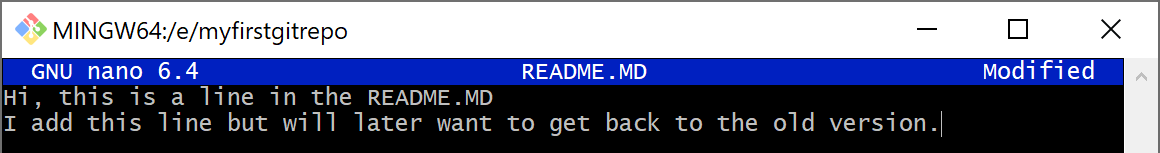
\includegraphics[width=\textwidth]{getback-2}
\end{center}

\end{frame}
 
\begin{frame}
\frametitle{Get back to earlier  versions 2}

\begin{center}
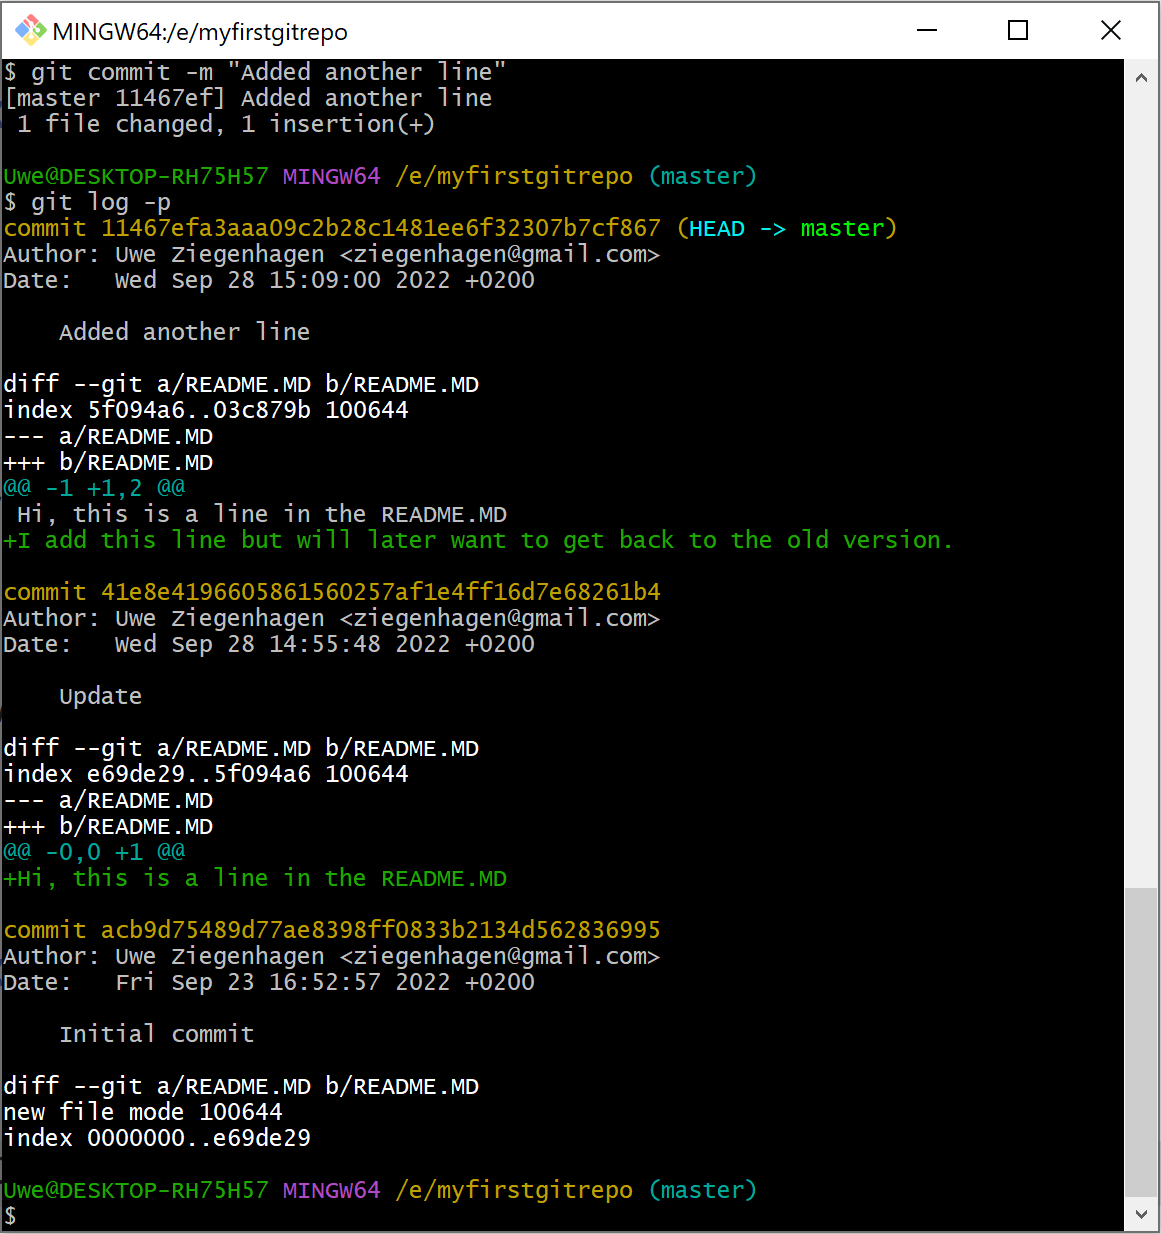
\includegraphics[width=0.7\textwidth]{getback-3}
\end{center}

\end{frame}

\begin{frame}
\frametitle{Get back to earlier versions 3}

To which version you want to go? 

\begin{center}
\fbox{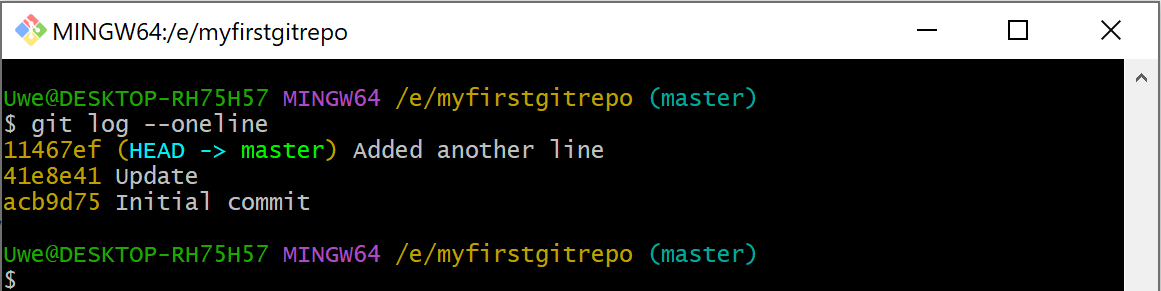
\includegraphics[width=\textwidth]{getback-4}}
\end{center}

\begin{itemize}
\item \texttt{git checkout 41e8e41 .}
\item Do not forget the dot at the end, otherwise you end in \texttt{detached head state}, which you can/need to fix by \texttt{git checkout master}
\end{itemize}

\end{frame}

\begin{frame}
\frametitle{Get back to earlier versions 4}

\begin{center}
\fbox{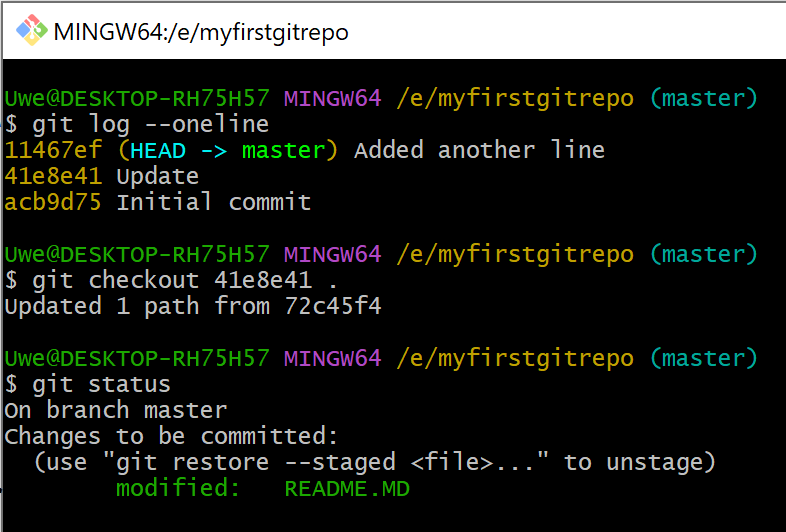
\includegraphics[width=0.75\textwidth]{getback-5}}
\end{center}

Commit this version as well and note in the message why you reverted!

\end{frame}

\begin{frame}
\frametitle{Get back to earlier versions 5}

\begin{center}
\fbox{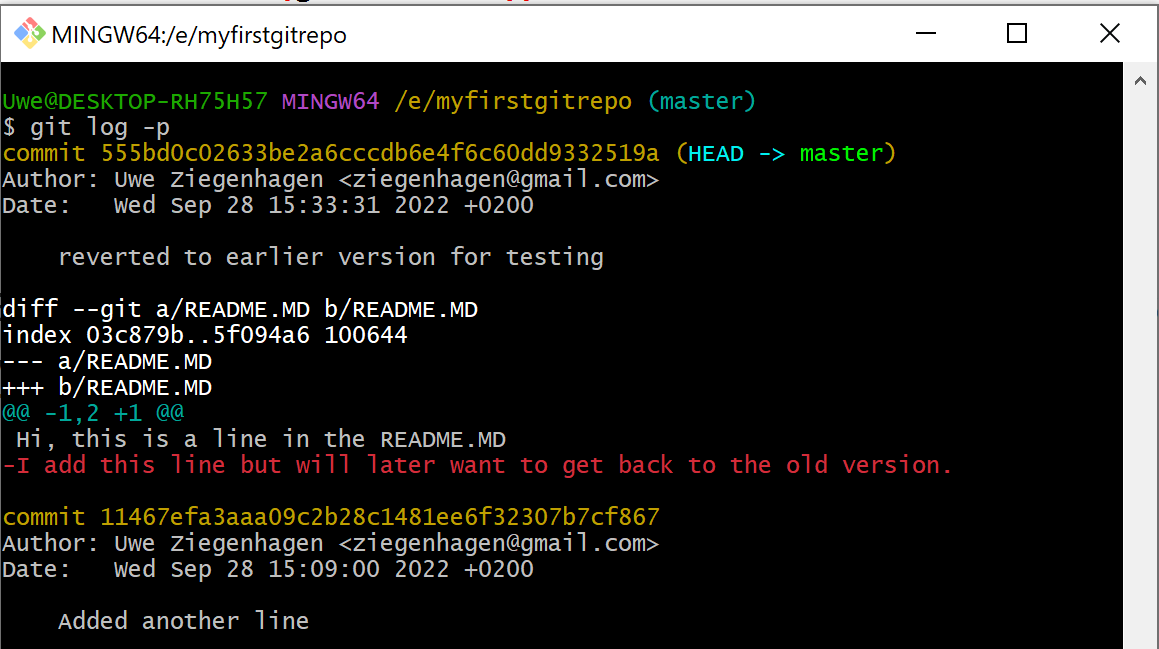
\includegraphics[width=\textwidth]{getback-6}}
\end{center}

\end{frame}


\end{document}